
\section{Results and Discussion}
\label{sec:Results}

\md{In order to evaluate the impacts of different components of our hybrid system, a series of experiments are conducted. We first show the re-projection error of different methods and then use a plaster human head as the ground truth to verify the quality of the 3D reconstruction result. Finally we show the reconstructed human body colored by different colors to }


\subsection{Re-projection error}
\xj{Why do we need reprojection error while the goal is 3D reconstruction? }
\md{The re-projection error describes the accuracy of the calibration result. We compute the re-projection and compare it to evaluate the effectivity of our global calibration step.}
Using the 2D coordinates of the corners detected in the checkerboard images, we can achieve the 3D space coordinates $\mathbf{P_{c}}$ by triangulation. Then we re-project $\mathbf{P_{c}}$ to each view which the checkerboard can be seen using the extrinsic parameters obtained by different methods and compute the average re-projection error, as shown in Table 1.
\begin{table*}
	\centering
	\caption{Average re-projection error (pixels) of each camera using different methods. (a) results by Kalibr ~\cite{Maye2013Self}, (b) results by Kalibr ~\cite{Maye2013Self} with our registration step, (c) results by our global calibration method, (d) results by our integrated method. The re-projection error of (c) is the smaller and uniform in each view, while the results of other methods contain the accumulative error and the inconsistence. }
	\label{tab:reprojection}
	\begin{tabular}{lcccccccc}
		\hline
		Methods & Cam 1 & Cam 2 & Cam 3 & Cam 4 & Cam 5 & Cam 6 & Cam 7 & Cam 8\\
		\hline
		(a) Kalibr &4.54 &3.20 &11.16 &10.74 &4.87 &6.75 &3.64 &5.11\\

		(b) Kalibr+ICP &3.75 &4.04 &11.40 &7.91 &6.39 &5.62 &3.39 &5.74\\
		
		(c) SBA   &\textbf{0.32} &\textbf{0.32} &\textbf{0.38}  &\textbf{0.35} &\textbf{0.37} &\textbf{0.40} &\textbf{0.33} &\textbf{0.34} \\
		
		(d) SBA+ICP &0.92 &0.99 &1.58 &2.19 &3.06 &1.79 &2.68 &1.38\\
		\hline
		
	\end{tabular}


\end{table*}


The reprojection error of the proposed global calibration method is the smaller among the different methods, which proves that the global optimization is quite effective. Although the registration step makes the model closer to the ground truth, it leads to the bigger reprojection error. That is because the aim of the registration step is to minimize the error caused by the inaccurate depth estimation, but not to optimize the camera parameters.


\subsection{Comparison with the ground truth}

\xj{Explain why do you need this experiment.}
\md{Due to the goal of our system is to achieve high-quality reconstruction model, we compare the results reconstructed by different methods with the ground truth.} 

A plaster model of a human head is placed in the center of our multi-camera system and the RGB and depth images of it can be obtained.
We scan the model using a 3D laser scanner and achieved a mesh of the plaster head with the error smaller than 0.04 mm.
We consider the accurate mesh as the ground truth and compare it with the reconstructed 3D model using different methods.
We compute the L2 distances of the point cloud to the mesh for each method. \md{For each point in the point cloud, we find the nearest point to it on the mesh, and compute the distance.} 
\xj{How do you compute the L2 distance between a point cloud and a mesh? for each point in a point cloud, find the nearest point on the mesh?}
%
The average error is listed in Table~\ref{fig:distance}. As we can see, our method has the smaller error, which proves that it can achieve a high-quality model.
We also show the distribution histogram of the error using different extrinsic parameters in Figure~\ref{fig:histogram}.
\xj{Fig 3?}
Similarly, the result of our method has the more accurate result.

\begin{figure*}[ht]
  \centering
\subfigure[]{
\begin{minipage}[c]{.22\linewidth}
\centering
  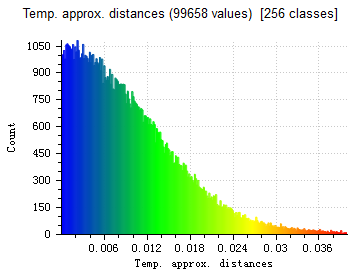
\includegraphics[width=4cm]{image/dis_1.png}
\end{minipage}
}%
\subfigure[]{
\begin{minipage}[c]{.22\linewidth}
\centering
  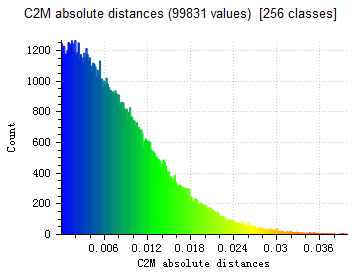
\includegraphics[width=4cm]{image/dis_2.png}
\end{minipage}
}
\subfigure[]{
\begin{minipage}[c]{.22\linewidth}
\centering
  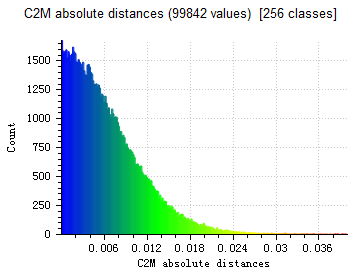
\includegraphics[width=4cm]{image/dis_3.png}
\end{minipage}
}
\subfigure[]{
\begin{minipage}[c]{.22\linewidth}
\centering
  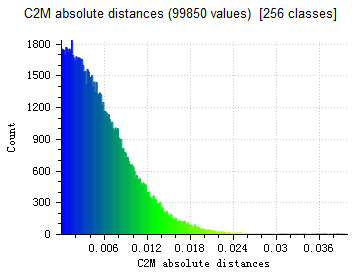
\includegraphics[width=4cm]{image/dis_4.png}
\end{minipage}
}
\caption{The distribution histogram of the L2 distances of the point cloud reconstructed using different methods to the ground truth. (a) results by Kalibr ~\cite{Maye2013Self}, (b) results by Kalibr ~\cite{Maye2013Self} with our registration step, (c) results by our global calibration method, (d) results by our integrated method. The number of the points with small distance increases obviously after the optimization and registration step we proposed.}
\label{fig:histogram}
\end{figure*}

\subsection{Reconstruction results of human bodies}

We reconstruct the 3D point clouds of a human body standing in the center of our multi-camera system using various methods. \md{We mark the point cloud in different views with different colors to show the quality of the fusion results. Figure~\ref{fig:pointcloud} shows the results which demonstrate our algorithm. As we can see, the model reconstructed by our hybrid system has the highest quality.}
\xj{explain the results. show different views. }.

\xj{Show at least three groups of results, in different human pose.}

\begin{figure*}[ht]
  \centering
\subfigure[]{
\begin{minipage}[c]{.22\linewidth}
\centering
  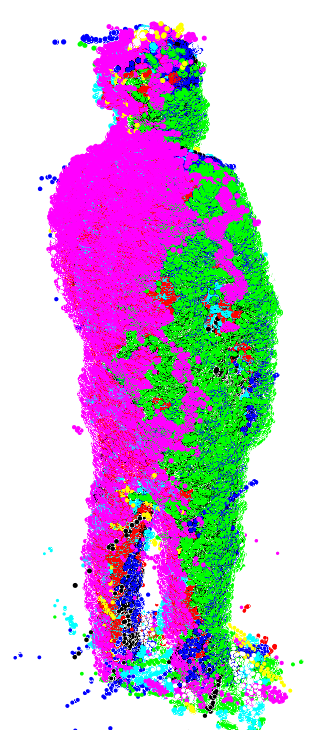
\includegraphics[width=2.5cm]{image/pc_1.png}
\end{minipage}
}%
\subfigure[]{
\begin{minipage}[c]{.22\linewidth}
\centering
  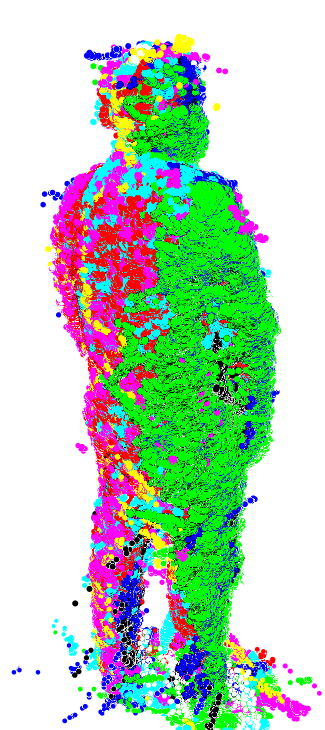
\includegraphics[width=2.5cm]{image/pc_2.png}
\end{minipage}
}
\subfigure[]{
\begin{minipage}[c]{.22\linewidth}
\centering
  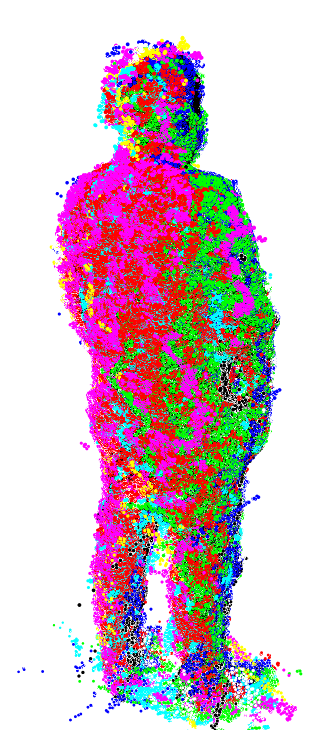
\includegraphics[width=2.5cm]{image/pc_3.png}
\end{minipage}
}
\subfigure[]{
\begin{minipage}[c]{.22\linewidth}
\centering
  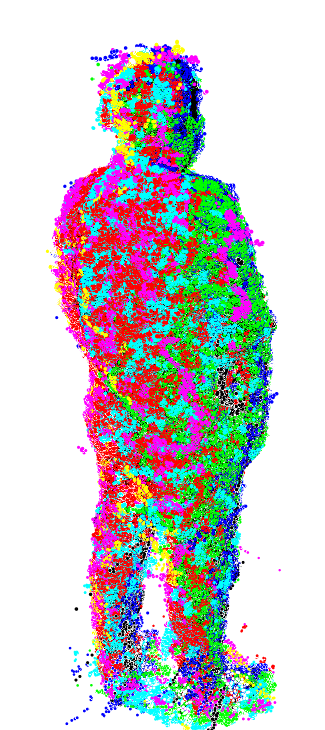
\includegraphics[width=2.5cm]{image/pc_4.png}
\end{minipage}
}
\caption{The reconstruction results of the back of a human using various methods.(a) results by Kalibr ~\cite{Maye2013Self}, (b) results by Kalibr ~\cite{Maye2013Self} with our registration step, (c) results by our global calibration method, (d) results by our integrated method. We render the point clouds with different colors to distinguish which view the point clouds belong to. The point clouds in result (a) are distinctly separated from other views, as the pink and green views cover the whole surface of the model. Result (b) becomes a little better while the green view still covers the right side of the body. The point clouds align quite well in result (c) with small blemishes, the azure view is inside the model. (d) shows a well-aligned model. }
\label{fig:pointcloud}
\end{figure*}


\begin{figure*}[ht]
  \centering
\subfigure[]{
\begin{minipage}[c]{.22\linewidth}
\centering
  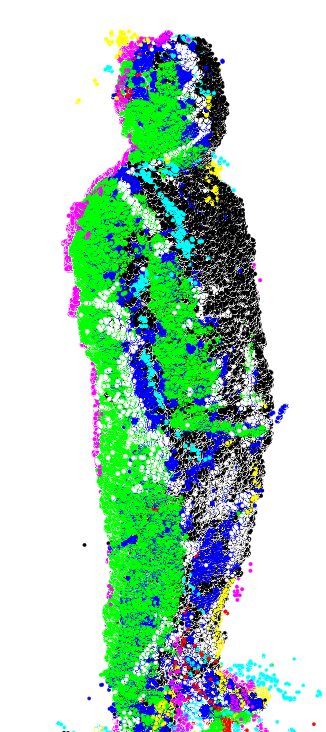
\includegraphics[width=2.5cm]{image/pc_1_1.png}
\end{minipage}
}%
\subfigure[]{
\begin{minipage}[c]{.22\linewidth}
\centering
  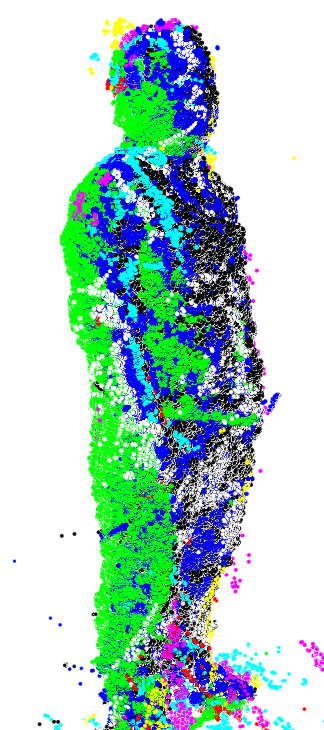
\includegraphics[width=2.5cm]{image/pc_2_1.png}
\end{minipage}
}
\subfigure[]{
\begin{minipage}[c]{.22\linewidth}
\centering
  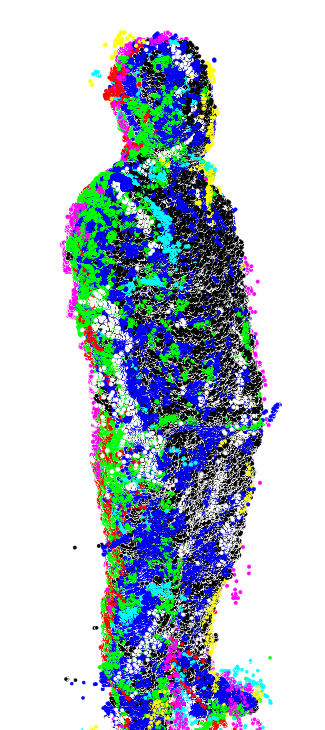
\includegraphics[width=2.5cm]{image/pc_3_1.png}
\end{minipage}
}
\subfigure[]{
\begin{minipage}[c]{.22\linewidth}
\centering
  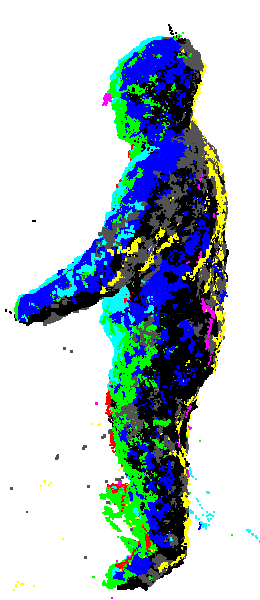
\includegraphics[width=2.5cm]{image/pc_4_1.png}
\end{minipage}
}
\caption{The reconstruction results of the back of a human using various methods.(a) results by Kalibr ~\cite{Maye2013Self}, (b) results by Kalibr ~\cite{Maye2013Self} with our registration step, (c) results by our global calibration method, (d) results by our integrated method.}
\label{fig:pointcloud}
\end{figure*}

\begin{figure*}[ht]
  \centering
\subfigure[]{
\begin{minipage}[c]{.22\linewidth}
\centering
  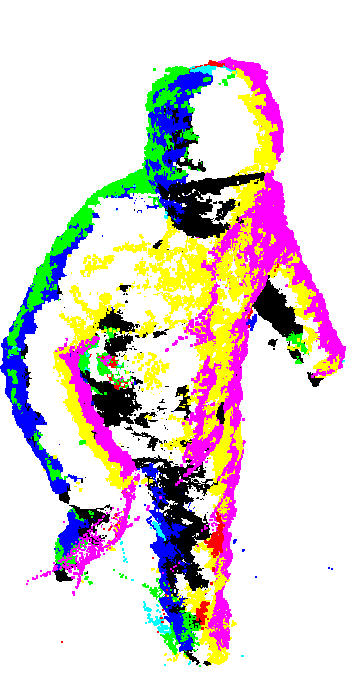
\includegraphics[width=2.5cm]{image/pc_1_2.png}
\end{minipage}
}%
\subfigure[]{
\begin{minipage}[c]{.22\linewidth}
\centering
  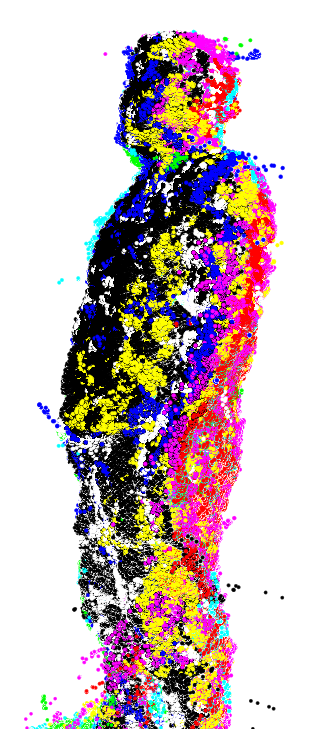
\includegraphics[width=2.5cm]{image/pc_2_2.png}
\end{minipage}
}
\subfigure[]{
\begin{minipage}[c]{.22\linewidth}
\centering
  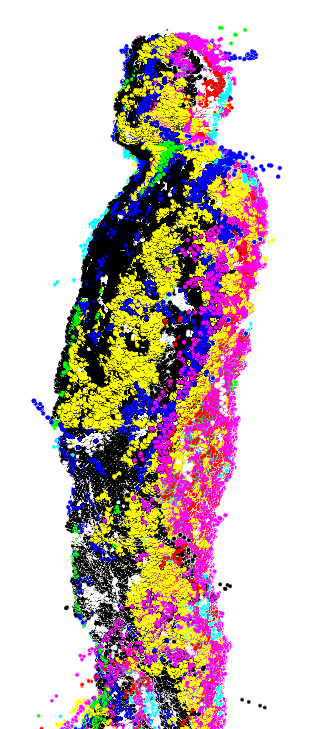
\includegraphics[width=2.5cm]{image/pc_3_2.png}
\end{minipage}
}
\subfigure[]{
\begin{minipage}[c]{.22\linewidth}
\centering
  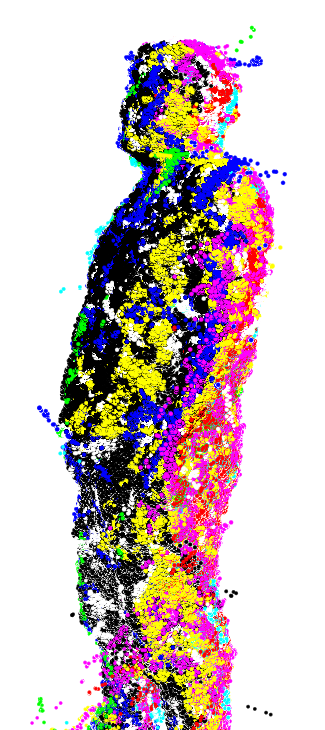
\includegraphics[width=2.5cm]{image/pc_4_2.png}
\end{minipage}
}
\caption{The reconstruction results of the back of a human using various methods.(a) results by Kalibr ~\cite{Maye2013Self}, (b) results by Kalibr ~\cite{Maye2013Self} with our registration step, (c) results by our global calibration method, (d) results by our integrated method.}
\label{fig:pointcloud}
\end{figure*}
\section{conclusion}
We present an efficient system integrating the multi-camera calibration and point cloud registration. By a global bundle adjustment, we reduce the accumulative error and the inconsistence caused by the pairwise camera pose estimation, and achieve a set of accurate extrinsic parameters with less reprojection error. With the point cloud registration, we minimize the error from the depth estimation and achieve a high-quality 3D model. Our calibration algorithm has been tested on both reprojection error and ground truth data. The experimental results has proved that the two steps of our system are both necessary and effective, and a more accuracy model can be reconstructed using our method.
\begin{table}
	\centering
	\caption{The distance between the point cloud and the ground truth. The distance (in centimeters )of the point cloud to the mesh of the plaster model computed by four different methods. (a) results by Kalibr ~\cite{Maye2013Self}, (b) results by Kalibr ~\cite{Maye2013Self} with our registration step, (c) results by our global calibration method, (d) results by our integrated method.}
	\label{tab:distance}
	\begin{tabular}{lcccc}
		\hline
		Methods & Mean &Standard deviation\\
		\hline
		(a) &0.9542 &0.7240\\

		(b) &0.8243 &0.6376\\
		
		(c) &0.6408 &0.5072\\
		
		(d) &0.5811 &0.4650\\
		\hline
		
	\end{tabular}
\label{fig:distance}
\end{table}


